\documentclass[12pt]{article}
\usepackage{amsmath}
\usepackage{graphicx}
\usepackage[export]{adjustbox}
\usepackage[bottom=0.2in]{geometry}

\begin{huge}
\title{Correlation Heatmaps of Earthquake Event vs. Solar Activity Variables}
\author{Zane van Campfort and Roman Avery}

\date{09/12/21}
\end{huge}
\setlength{\topmargin}{-1in}

\begin{document}
\maketitle
\begin{large}
Variables used:

\begin{itemize}
  \item magAFV - Magnitude of average field vector
  \item sB - sigma B (magnetic field)
  \item PT - Proton temperature
  \item PD - Proton density
  \item PFS - Plasma (flow) speed
  \item FP - Flow pressure
  \item EF - Electric field
  \item Kp - Planetary geomagnetic activity index
  \item DST - DST Index
\end{itemize}
\end{large}

\graphicspath{{../plots/09_12/}}


\newpage

\begin{figure}
\begin{large}
\title{Earthquake Magnitude vs. Solar Activity Variables}
\end{large}
\centering
  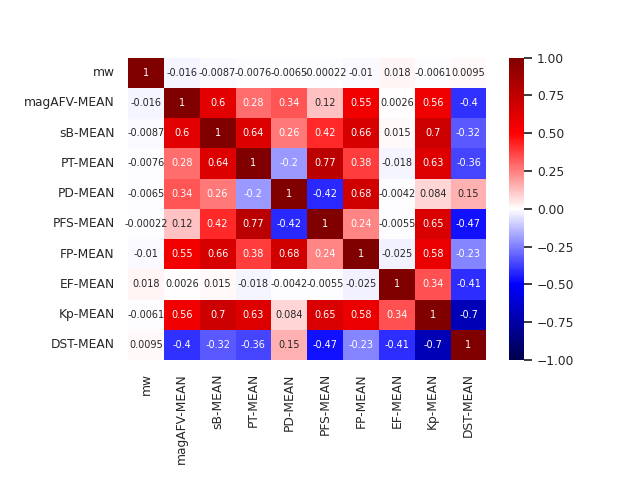
\includegraphics[width=0.95\textwidth]{corr-mw-MEAN.png}
  \caption{Earthquake Magnitude vs. SW Mean Values}

  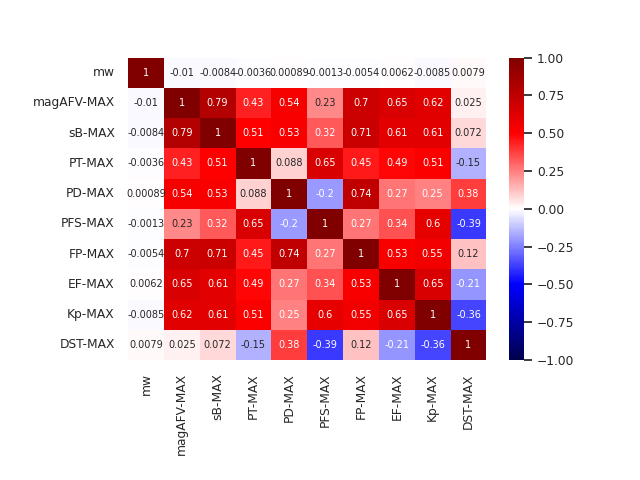
\includegraphics[width=0.95\textwidth]{corr-mw-MAX.png}
  \caption{Earthquake Magnitude vs. SW Max Values}
\end{figure}

\newpage

\begin{figure}
\centering
  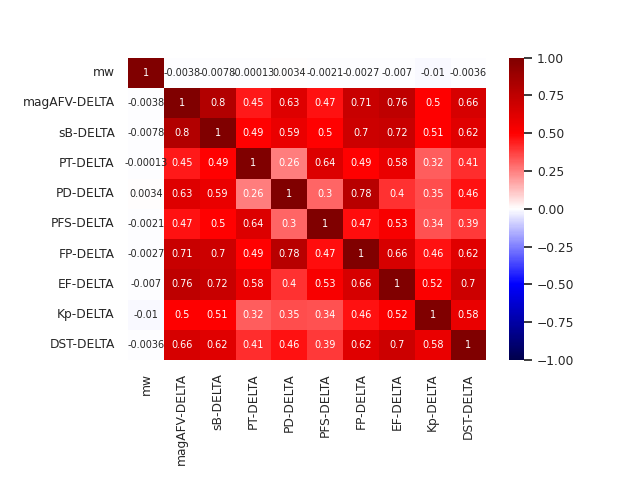
\includegraphics[width=0.95\textwidth]{corr-mw-DELTA.png}
  \caption{Earthquake Magnitude vs. SW Change in Values}

  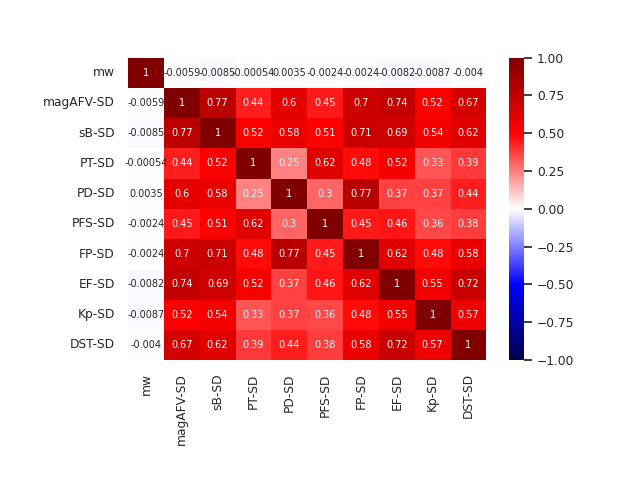
\includegraphics[width=0.95\textwidth]{corr-mw-SD.png}
  \caption{Earthquake Magnitude vs. SW Value Standard Distributions}

\end{figure}

\newpage

\begin{figure}
\begin{large}
\title{Earthquake Depth vs. Solar Activity Variables}
\end{large}
\centering
  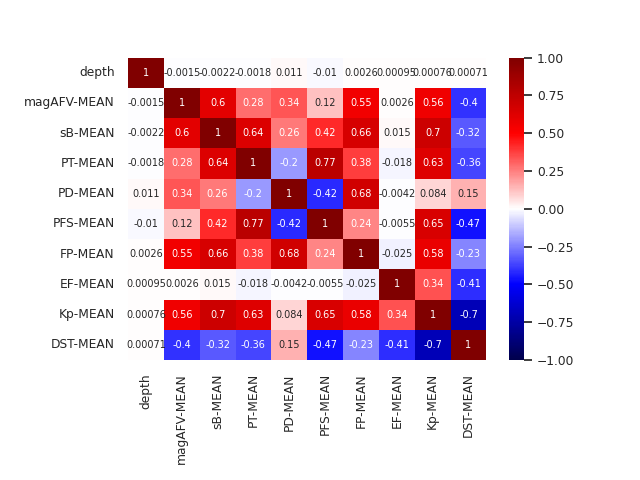
\includegraphics[width=0.95\textwidth]{corr-depth-MEAN.png}
  \caption{Earthquake Depth vs. SW Mean Values}

  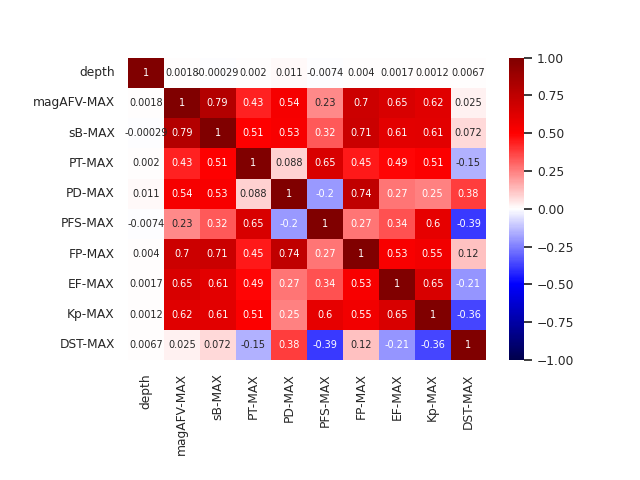
\includegraphics[width=0.95\textwidth]{corr-depth-MAX.png}
  \caption{Earthquake Depth vs. SW Max Values}
\end{figure}

\newpage

\begin{figure}
\centering
  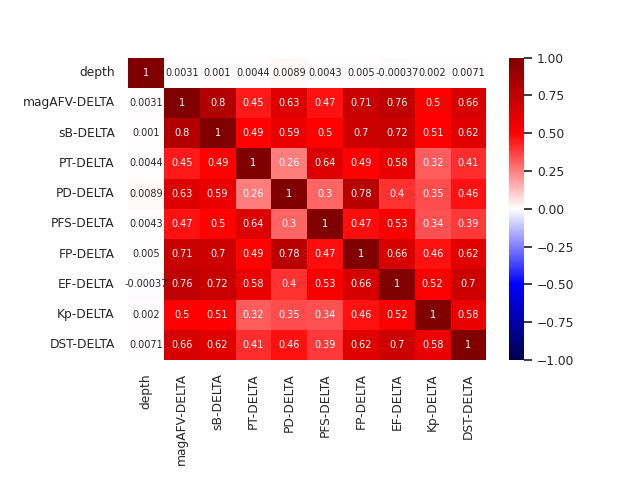
\includegraphics[width=0.95\textwidth]{corr-depth-DELTA.png}
  \caption{Earthquake Depth vs. SW Change in Values}

  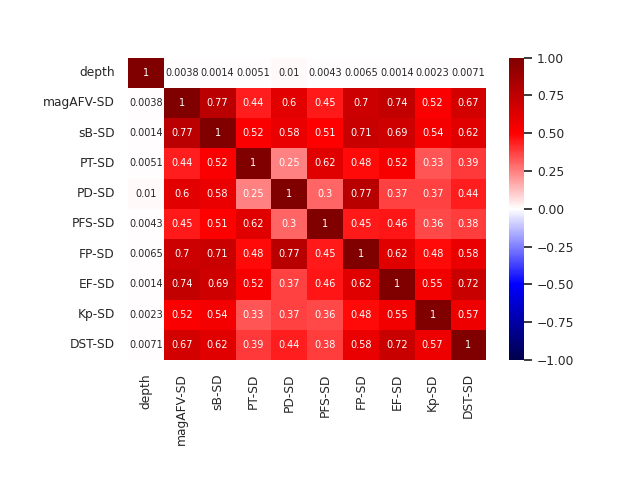
\includegraphics[width=0.95\textwidth]{corr-depth-SD.png}
  \caption{Earthquake Depth vs. SW Value Standard Distributions}

\end{figure}

\newpage

\begin{figure}
\begin{large}
\title{Earthquake Latitude vs. Solar Activity Variables}
\end{large}
\centering
  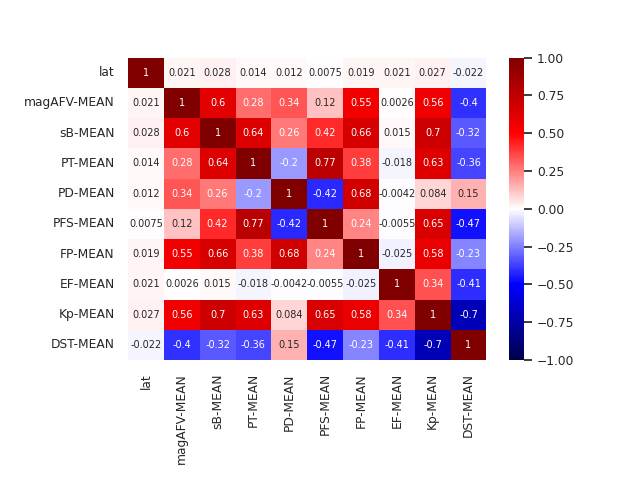
\includegraphics[width=0.95\textwidth]{corr-lat-MEAN.png}
  \caption{Earthquake Latitude vs. SW Mean Values}

  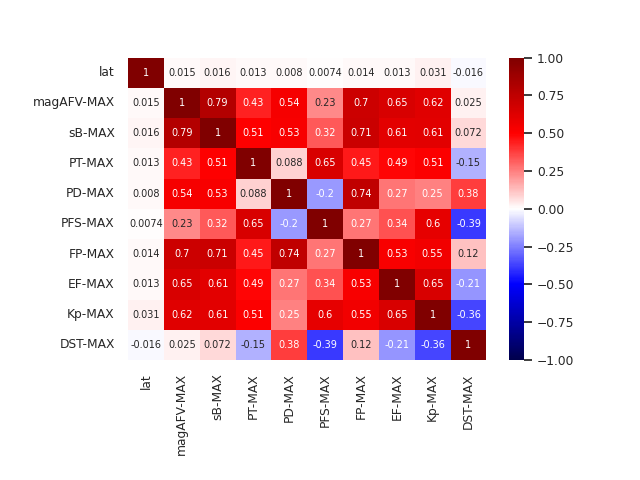
\includegraphics[width=0.95\textwidth]{corr-lat-MAX.png}
  \caption{Earthquake Latitude vs. SW Max Values}
\end{figure}

\newpage

\begin{figure}
\centering
  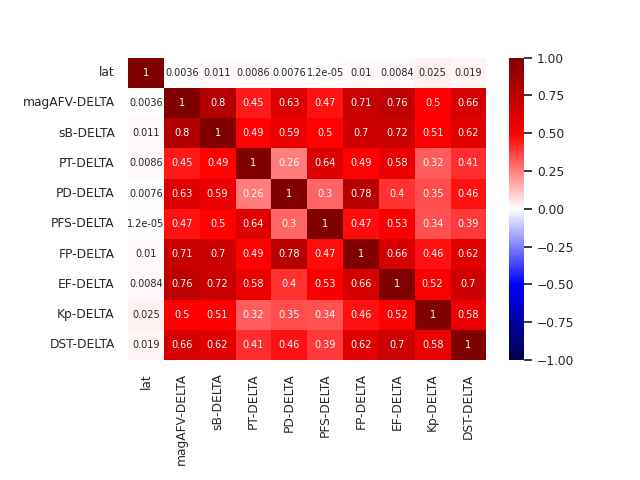
\includegraphics[width=0.95\textwidth]{corr-lat-DELTA.png}
  \caption{Earthquake Latitude vs. SW Change in Values}

  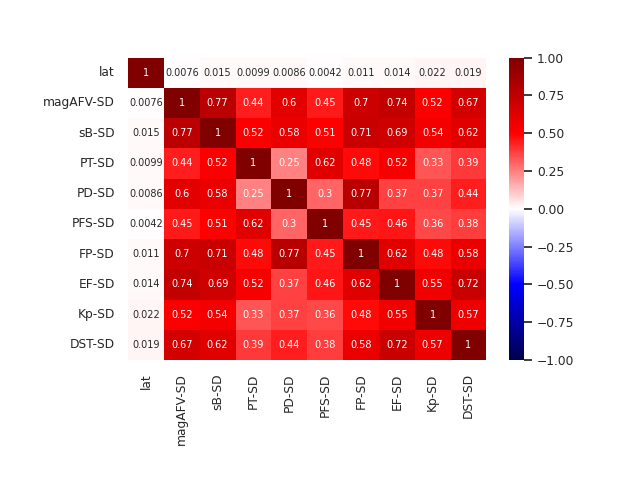
\includegraphics[width=0.95\textwidth]{corr-lat-SD.png}
  \caption{Earthquake Latitude vs. SW Value Standard Distributions}

\end{figure}

\newpage

\begin{figure}
\begin{large}
\title{Earthquake Longitude vs. Solar Activity Variables}
\end{large}
\centering
  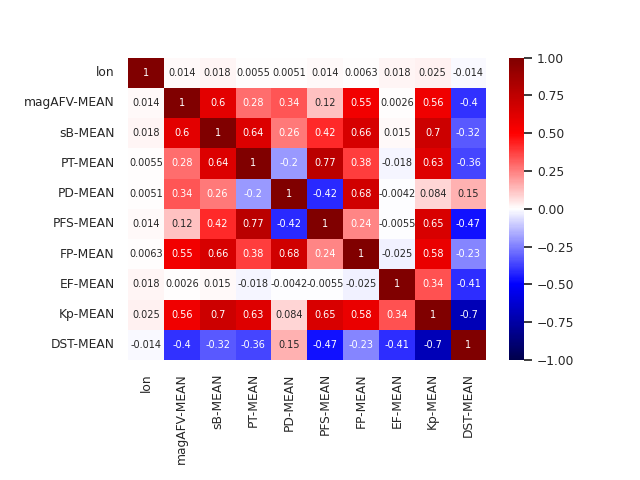
\includegraphics[width=0.95\textwidth]{corr-lon-MEAN.png}
  \caption{Earthquake Longitude vs. SW Mean Values}

  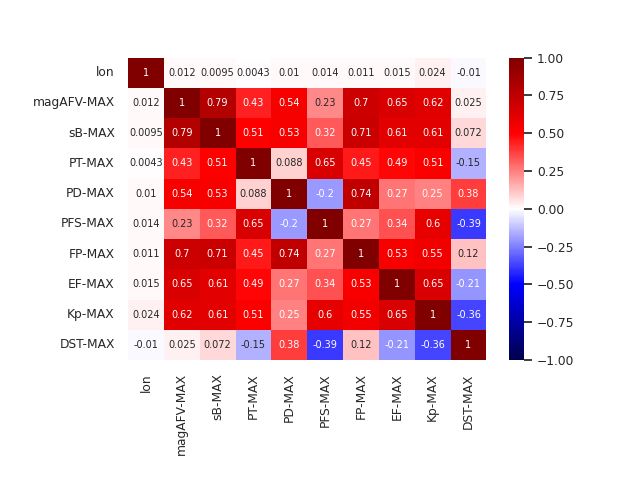
\includegraphics[width=0.95\textwidth]{corr-lon-MAX.png}
  \caption{Earthquake Longitude vs. SW Max Values}
\end{figure}

\newpage

\begin{figure}
\centering
  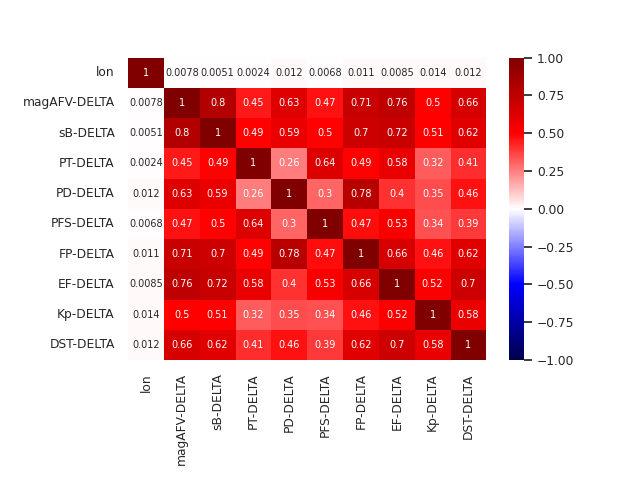
\includegraphics[width=0.95\textwidth]{corr-lon-DELTA.png}
  \caption{Earthquake Longitude vs. SW Change in Values}

  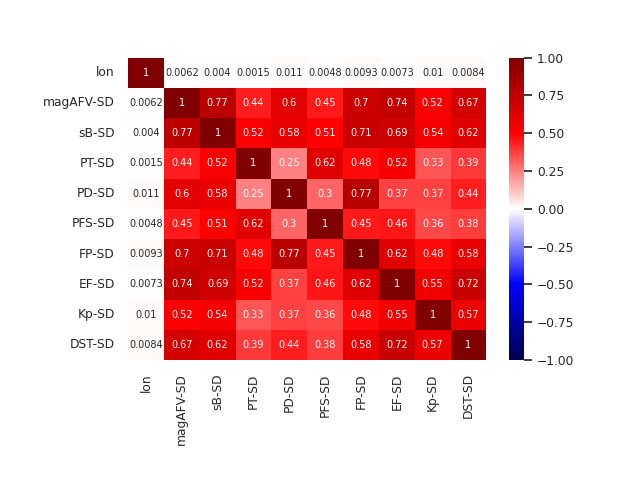
\includegraphics[width=0.95\textwidth]{corr-lon-SD.png}
  \caption{Earthquake Longitude vs. SW Value Standard Distributions}

\end{figure}

\newpage

\end{document}